\documentclass[10pt]{article}

\usepackage[utf8]{inputenc}
\usepackage{floatrow}

\usepackage{algorithm}
\usepackage{algorithmic}
\usepackage[T1]{fontenc}
\usepackage{enumitem}
\usepackage{hyperref}
\usepackage{graphicx}
\usepackage{color}
\usepackage{listings}
\usepackage{wrapfig}
\usepackage[hmargin=1.25in,vmargin=1.25in]{geometry}

%title setup
\title{Projet IPI: chemins de poids minimum}
\author{Romain PEREIRA}
\date{04/12/2017}

% table of contents setup
\renewcommand{\contentsname}{Sommaire}
\usepackage{etoolbox}
\patchcmd{\thebibliography}{\section*{\refname}}{}{}{}

\hypersetup{
    colorlinks,
    citecolor=black,
    filecolor=black,
    linkcolor=blue,
    urlcolor=red
}
			
\begin{document}
	\maketitle
	\tableofcontents

	\section*{Préambule}

		Ce projet est réalisé dans le cadre de mes études à l'ENSIIE. Le but est d'implémenter des
		algorithmes de recherche de 'chemin le plus court' dans des graphes orientés.
		Ce document rapporte mon travail, et explique les choix techniques qui ont été pris.
		Soit (X, A) un graphe. On note:
				
		\begin{itemize}[label=-]
			\setlength\itemsep{0.1em}
			\item X : sommets du graphe
			\item A : arcs du graphe
			\item n : Card(X)
			\item s : sommet 'source', celui à partir duquelle les chemins sont construits
			\item t : sommet 'target', celui vers lequel on souhaite construire un chemin
		\end{itemize}

		\begin{figure}
			\floatbox[{\capbeside\thisfloatsetup{capbesideposition={right,top},capbesidewidth=6cm}}]{figure}[\FBwidth]
			{\caption{\textit{\newline graphe G n=7, \newline X=\{1, 2, ... 7\}, \newline A=\{(1, 4), (4, 6), ... (6, 7)\}}}
			\label{graphe}}
			{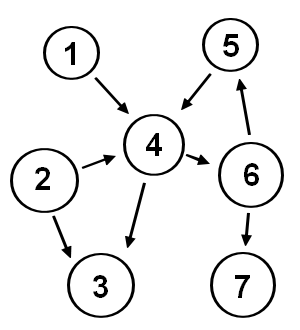
\includegraphics[height=2.5cm]{./images/graph.png}}
		\end{figure}

	\newpage
	\section{Recherche de chemin le plus court}
		\subsection{Parcours en largeur (graphes non-pondérés)}
			On considère ici un graphe où les arcs sont non pondérés. 'Le chemin le plus court'
			entre 2 sommets correspond à une famille d'arcs, dont le cardinal est minimum.
			On souhaite coder l'information:
			\begin{itemize}[label=-]
				\item `il existe un arc entre le sommet 'u' et le sommet 'v' `
			\end{itemize}
			
			\subsubsection{1ère approche}

				Cette information est un booléen, et peut donc être codée sur un bit.
				Soit 'b' l'indice d'un bit dans un tableau d'octet.
				Pour y accéder, il faut récuperer l'indice $\textrm{b}_\textrm{o}$ de l'octet correspondant dans le tableau,
				et l'indice $\textrm{b}_\textrm{b}$ du bit sur cet octet.\newline
				
				\begin{wrapfigure}{R}{5cm}
					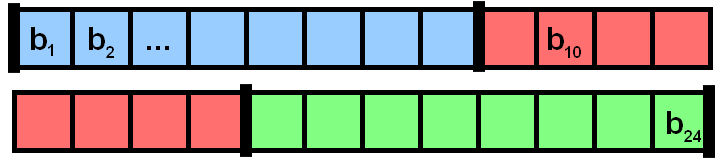
\includegraphics[width=5cm]{./images/bits.png}
					\caption{\textit{Schéma bits}}
				\end{wrapfigure}
				
				En posant:
				\begin{itemize}[label=-]
					\item \(b_o = b / 8\) (quotient de la division euclidienne de 'b' par 8)
					\item \(b_b = b \% 8\) (reste de la division euclidienne de 'b' par 8)
				\end{itemize}
				on s'assure de l'unicité,
				\begin{itemize}[label=-]
					\item \(b = 8*b_o+b_b\)
				\end{itemize}
				De plus, étant donné deux sommets 'u' et 'v', en posant
				\begin{itemize}[label=-]
					\item \(b = n * v + u\)
				\end{itemize}
				on peut cartographier les arcs sur le tableau de bits. Le bit vaut alors 1 s'il existe un arc entre 'u' et 'v', 0 sinon.
				On a besoin de \(n^2\) bits, et donc de \(n^2 / 8 + 1\) octets.
				On utilise donc 8 fois moins de mémoire que si l'information était stockée sur un octet.
				De plus, on ne perds pas (ou très peu) de temps en lecture / écriture, car ces changements
				de coordonnées ne nécessite que 1 multiplication, 1 addition, et quelques opérations sur les bits (diviser par 8 <=> décaler
				les bits de 3 vers la droite)
				
				Egalement, en réduisant la mémoire utilisée, le programme est rendu plus `cache-friendly` \cite{cache_friendly},
				lorsque l'on teste le voisinnage entre 2 arcs en parcourant la matrice.\newline
				 
			\subsubsection{2ème approche}
				La complexité ('spatiale') de stockage des arcs est donc en \(1/8*O(n^2)\).
				Plus précisement, pour \(n=10^6\) (cas labyrinthe exo3/tests/06),
				l'espace mémoire nécessaire est de \(125Go\)... On va donc changer de structure de données.
				En ajoutant un attribut liste à chaque sommet, qui contient l'indice de ses sommets voisins,
				la complexité spatiale devient donc (au plus) en \(m * O(n)\), où 'm' est
				le nombre maximal de successeurs par sommet. (Remarque : pour \(m = n\), on retrouve \(O(n^2)\))
				Il en résulte que dans la résolution de labyrinthe (exo3/tests/06), on a \(m <= 5\), donc pour \(n=10^6\),
				on passe donc de \(125Go\) à \(5 Mo\). Les transformations précèdentes vont cependant être ré-utilisées
				dans Dijkstra et A*.
				
			\subsubsection{Algorithme de remontée}

				\begin{wrapfigure}{R}{5cm}
					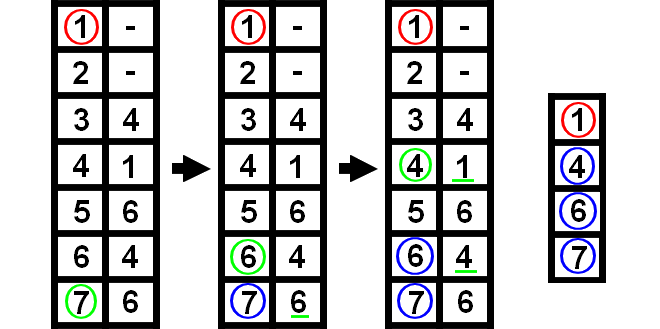
\includegraphics[width=5cm]{./images/remonte.png}
					\caption{\textit{Schéma de l'algorithme de remontée (voir Figure \ref{graphe})}}
				\end{wrapfigure}

				Chaque sommet 'u' du graphe possède un attribut pointant vers un autre sommet du graphe.
				Une fois l'algorithme de parcours terminé, cet attribut pointe vers le prédécesseur de 'u',
				dans le chemin le plus court allant de 's' à 'u'.
				Pour reconstruire le chemin, il suffit de regarder récursivement les prédécesseurs, en partant du sommet
				't' jusqu'à ce que l'on ait atteint 's'.
				La complexité de la reconstruction est en O(m), où 'm' est la longueur du chemin.\newline
				
				Cette modélisation permet de réduire les coûts de stockage, et la remontée est d'un coût
				négligeable devant le temps de résolution du chemin. Elle sera réutilisée dans Dijkstra et A*.
			
		\subsection{Algorithme de Dijkstra (graphes pondérés positivement)}
			On considère ici un graphe où les arcs sont pondérés avec des poids positifs.\newline
			'Le chemin le plus court' entre 2 sommets correspond au chemin avec la somme des poids de ses arcs minimum.\newline
			L'algorithme de Dijkstra nous est fourni dans le sujet. Remarquons que si le poids de tous les arcs sont identiques,
			on retrouve l'algorithme de parcours en largeur.
			\subsubsection{1ère approche}
				L'implémentation reprend le squelette du parcours en largeur.
				Cependant, une différence fondamentale réside dans le choix du prochain sommet à visiter.
				Dans le parcours en largeur, les sommets sont visités dans leur ordre d'apparition dans la liste (1er entré, 1er sorti).
				Trouver le prochain sommet à visiter est d'une complexité \(O(1)\).
				Dans l'algorithme de Dijkstra, les sommets sont visités par ordre du poids de leur chemin de 's'.
				Ainsi, on pourrait parcourir tous les sommets non-visités, et en extraire un minimum (dans le sens de sa distance à 's')
				Si la file contient 'm' sommets non visité, la complexité de cette opération est en \(O(m)\).
				
				Après avoir implementé Dijkstra avec cette 1ère approche, j'ai étudié le temps d'éxecution.
				\begin{figure}[H]
					\begin{center}
						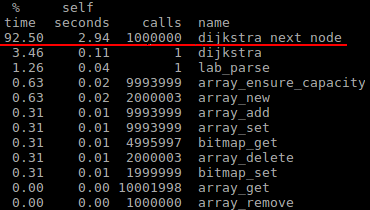
\includegraphics[width=6cm,height=\textheight,keepaspectratio]{./images/no_pqueue.png}
					\end{center}
				    \caption{\textit{résultat de 'gprof' sur 'tests/exo3/06'}}
				\end{figure}
				Il s'est avéré que mon programme passe (en moyenne) plus de 70\% de
				son temps d'éxecution à chercher le prochain sommet à visiter.
				(l'opération `trouver un sommet 'u' non visité minimisant d(u)` dans l'algorithme fourni).\newline

			\subsubsection{File de priorité ('Priority Queue')}

				Ainsi, j'ai decidé d'implémenter des 'files de priorités', et plus précisement des
				'tas binaires' \cite{binary_heap}, afin d'optimiser cette partie du programme.
				Cette structure de données est une file, permettant de définir des priorités parmis les éléments,
				et d'effectuer les 4 opérations élémentaires suivantes (avec 'm' le nombre d'éléments de la file):
				\begin{itemize}[label=-]
					\item 'insérer un élément' : \(O(log(m))\)
					\item 'extraire l'élément ayant la plus grande priorité' : \({O(log(m))}\)
					\item 'tester si la file de priorité est vide' : \(O(1)\)
					\item '\underline{diminuer} la priorité d'un élément déjà inséré' : \(O(log(m))\)
				\end{itemize}
				les détails techniques de cette structure peuvent être trouvés en annexe \cite{binary_heap},
				et son implementation dans les fichiers \textit{pqueue.[c,h]}.
				
				On passe alors d'une complexité \(O(n * m)\) à \(O(n * log(m))\) pour l'algorithme de Dijkstra.

				\begin{figure}[H]
					\begin{center}
						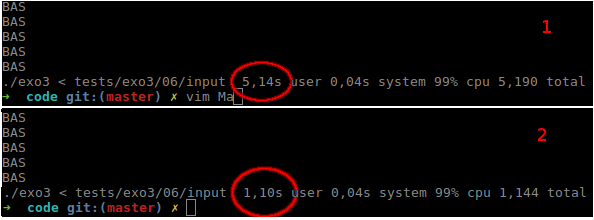
\includegraphics[width=11cm,height=\textheight,keepaspectratio]{./images/performances.png}
					\end{center}
					\caption{\textit{Temps d'éxecution avec et sans une file de priorité, sur le test exo3/06}}
				\end{figure}
				
				\begin{itemize}[label=-]
					\setlength\itemsep{0.1em}
					\item 1 : Dijkstra sans file de priorité
					\item 2 : Dijkstra avec file de priorité
				\end{itemize}

				Voici une courbe d'étude sur les performances de Dijkstra (avec file de priorité)
				\begin{figure}[H]
					\begin{center}
						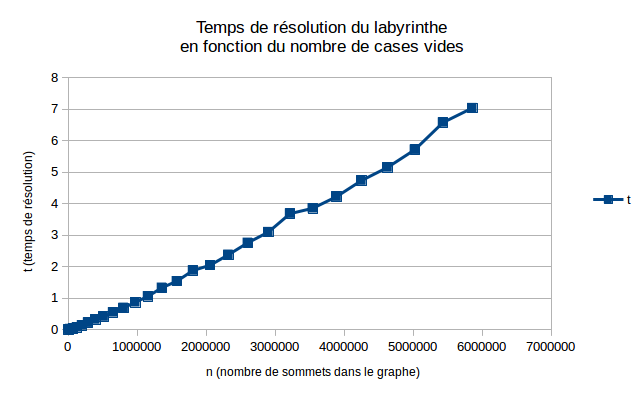
\includegraphics[height=6cm,keepaspectratio]{./images/courbe_temps.png}
					\end{center}
					\caption{\textit{Temps de résolution (en sec.) de labyrinthe avec Dijkstra, allure en \(O(n * log(m))\)}}
					\label{courbe_temps}
				\end{figure}

		\subsection{Algorithme A* (graphes pondérés et fonctions heuristiques)}
			L'algorithme A* est une extension de l'algorithme de Dijkstra \cite{computerphile_maze} \cite{computerphile_astar}.
			Avec l'algorithme de Dijkstra, on parcourt le graphe en largeur selon le poids de ses arcs.
			Avec A*, on effectue la même opération, mais on ajoute une heuristique \cite{heuristique} aux poids des arcs.\newline
			
			Cette heuristique permet de modifier l'ordre de priorité dans lequel les sommets seront visités dans le graphe.
			Bien qu'elle fait perdre l'optimalité, elle permet d'orienter la recherche dans le graphe, rendant la convergence vers
			un chemin plus rapide. (et avec une heuristique bien conçu au problème, on s'assure d'une solution acceptable).
			De plus, on peut très bien décider de laisser la recherche s'affiner, 
			Par exemple, dans la résolution de labyrinthe, une heuristique intéressante est la distance de Manhattan. \cite{manhattan}			
			Remarquons également qu'en utilisant une heuristique nulle (qui renvoie toujours '0'),
			on obtient très exactement l'algorithme de Dijkstra.

	\section{Application: résolution labyrinthe}
	
		\begin{wrapfigure}{R}{4.5cm}
			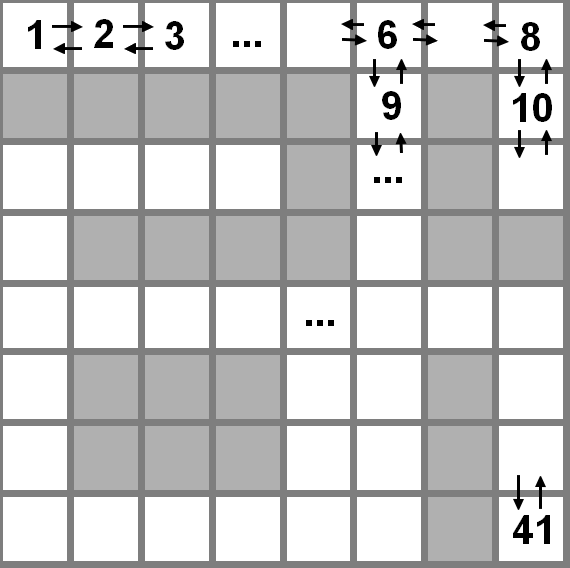
\includegraphics[width=4.5cm]{./images/lab.png}
			\caption{\textit{Modélisation du labyrinthe}}
			\label{modelisationlab}
		\end{wrapfigure}
		
		Dans l'exercice 3, on nous propose de résoudre des labyrinthes.\newline
		
		Intuitivement, le labyrinthe peut être modélisé par ce type de graphe (voir Figure \ref{modelisationlab}).
		On crée un sommet pour chaque case 'non-mur' (cases vides, téléporteurs, porte, clef).
		Pour chaque sommet, on crée des arcs entre lui et ses voisins.\newline
			
		\subsection{1ère approche} \label{first_approach}
			Une fois le labyrinthe modélisé, il ne reste plus qu'à le résoudre à l'aide des algorithmes préalablment implementés.\newline
			
			Cependant, cette approche demande de générer un graphe dans le bon format, et il s'est avéré que générer un telle
			en mémoire et en temps (requiet beaucoup de mémoires avec cette modélisation).
			La 1ère implementation est disponible dans le dossier '.bkp' de l'archive, on ne s'attardera pas dessus.

		\begin{wrapfigure}{R}{8cm}
			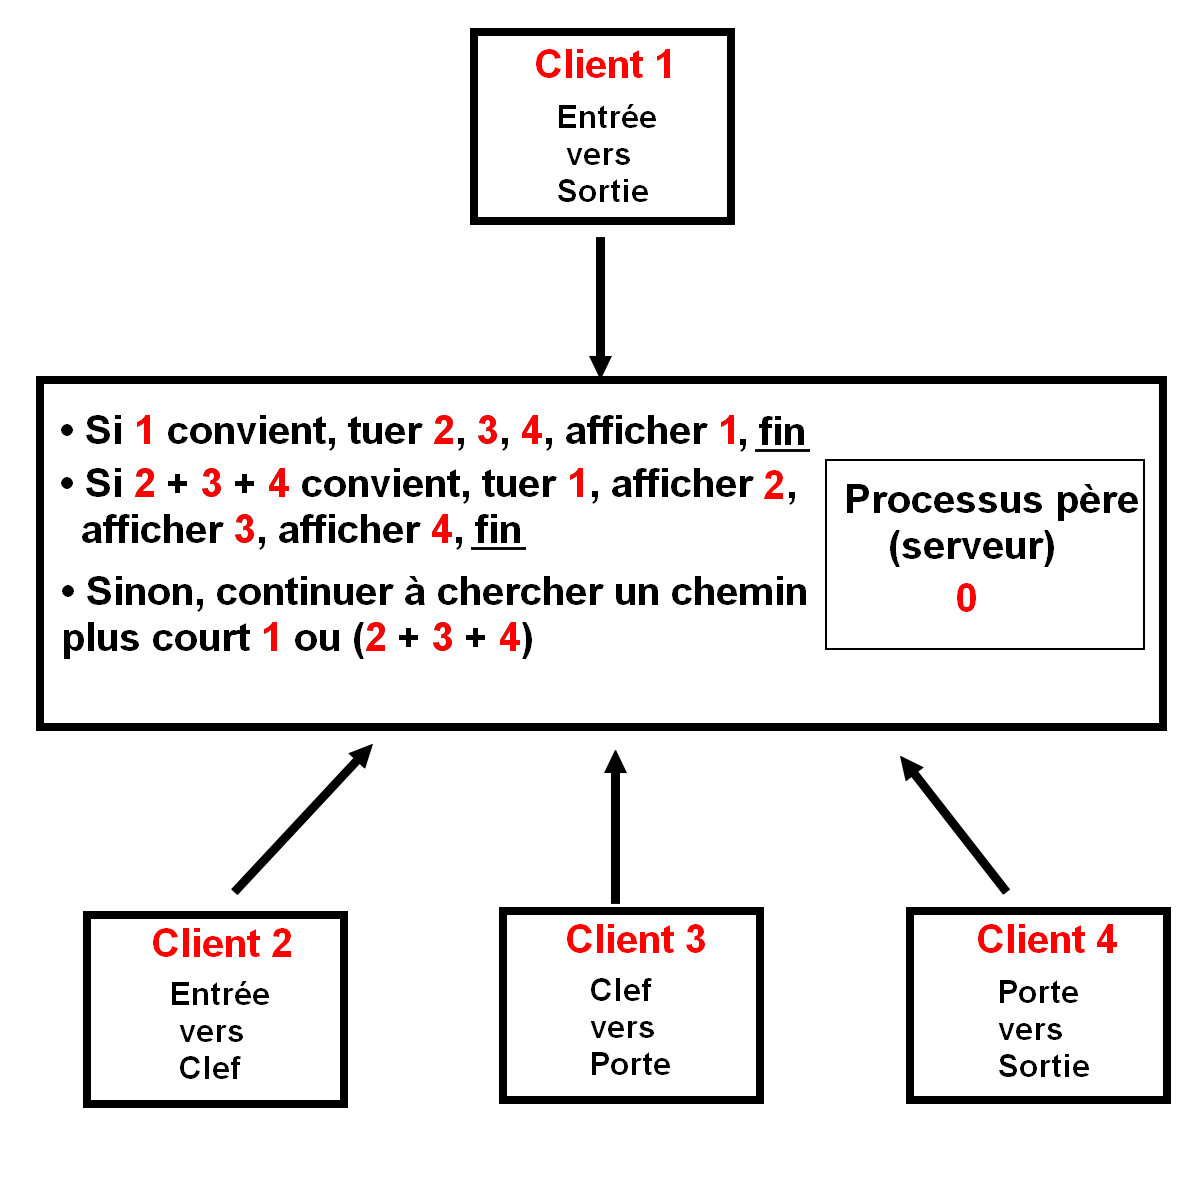
\includegraphics[width=8.0cm]{./images/exo3.png}
			\caption{\textit{Modèle client/serveur}}
			\label{exo3}
		\end{wrapfigure}

		\subsection{Optimisation} \label{ssec:optimisation}
			Après avoir ré-implementer A* specifiquement au problème, en travaillant directement sur la grille,
			voici les résultats obtenus:
			\begin{figure}[H]
				\begin{center}
					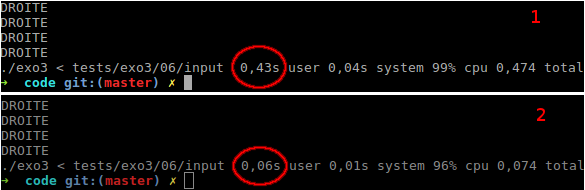
\includegraphics[width=10cm,height=\textheight,keepaspectratio]{./images/manhattan_performances.png}
				\end{center}
				\caption{\textit{performances sur 'tests/exo3/06'}}
			\end{figure}

			\begin{itemize}[label=-]
				\setlength\itemsep{0.1em}
				\item 1: (\ref{first_approach}) avec A* et la distance de Manhattan. : Le programme passe 90 (~ 0.4sec)\%
				de son temps à générer le graphe, 10\% (~0.05 sec) à résoudre.
				\item 2: (\ref{ssec:optimisation}) avec A* et la distance de Manhattan : le programme ne génère pas de graphes, il résout
				en travaillant sur la grille directement. (on utilise également 4 fois moins de mémoire qu'avec la 1ère approche).
			\end{itemize}

		\subsection{Parallélisation}
			Pour paralléliser la recherche, on crée un modèle 'client/serveur'.
			Le processus père est le 'serveur', et les processus fils sont les 'clients'.\newline

			Coté client, chaque processus calcule une partie du chemin à l'aide de l'algorithme A*
			une partie du chemin ((entrée, clef), (clef, porte), (porte, sortie))
			Dés qu'un chemin (ou un chemin plus court que le précèdent) est trouvé, il notifie le serveur
			en lui envoyant des données via un 'pipe'.\newline
			
			Coté serveur, le processus père ne fait que lire les chemins des clients, et essaye de trouver une
			solution en concaténant les chemins. Si une solution convient, il notifie ces clients (via des 'signaux')
			d'afficher leur chemin, et de s'arrêter.\newline
			
			Ce modèle n'est pas optimal. Par exemple, si un chemin est trivial, et que le client
			le trouve rapidement, il passera le reste du temps à attendre que les autres aient fini
			pour savoir s'il doit afficher son chemin ou non.\newline
			
			On aurait pu imaginer que dés qu'un processus ait fini, il aide un autre client à résoudre une autre partie du chemin
			(avec une autre heuristique par exemple, ou bien encore en divisant le chemin en 2 à l'aide d'un point subsidiaire à 'mi-chemin').
			Mais pour des raisons de simplicité, on reste sur ce modèle qui offre déjà de belles performances:
			
		\subsection{Critiques/limites}
		
			Bien que les performances obtenus remplisse le cahier des charges, il y a des limites dans cette modélisation.
			
			Premièrement, la distance de Manhattan n'est sans doute pas une bonne heuristique pour ce problème, car elle ne prends
			pas en compte la présence des téléporteurs.
			
			Deuxiemement, dans le pire des cas (c'est à dire, où A* ne converge pas rapidement, et devient equivalent à un parcours en largeur),
			le programme est plus lent (et plus couteux en mémoire!) que si l'on avait effectué un parcours en largeur.
			En effet, avec A*, l'opération 'passer au sommet suivant' est en \(O(log(m))\), avec 'm' le nombre de sommet dans la file de visite,
			alors qu'avec un parcours en largeur, cette opération est en \(O(1)\).
			Donc, si on doit parcourir tous les sommets, on a une complexité en \(O(n * log(m))\) (avec 'n' le nombre de sommet total, et
			'm' le nombre de sommet en moyenne dans la file), contre \(O(n)\) avec un parcours en largeur classique.

	\section{A propos de l'implémentation}
		Ci-joint, vous trouverez l'implémentation en language C.
		\subsection{Types / Structures de données}
		
		Les structures de données de manière générique, afin de pouvoir être ré-utilisé.
		(voir les fichiers '.c' et '.h', qui sont commentés). 

		\subsection{Qualité logiciel}
			Les programmes passent les tests fournis. Quelques tests supplémentaires ont également été créé pour mettre en défaut la résolution de labyrinthe,
			et pour illustrer ce document. (notamment pour l'illustration \ref{courbe_temps})\newline
			De plus, l'intégralité du code a été debogguer à l'aide de l'outil 'valgrind'.
			Il ne semble y avoir ni fuite mémoire, ni dépassement de tampon, ni accès à de la mémoire non initialisée.
			(avec des fichiers bien formattés du moins).
			\begin{figure}[H]
				\begin{center}
					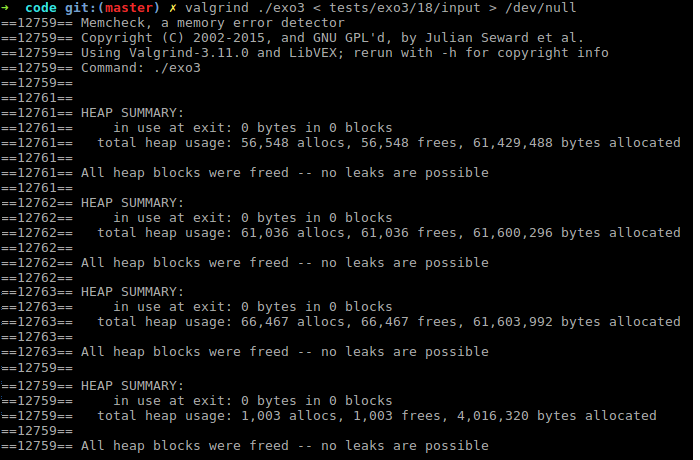
\includegraphics[width=12cm,height=\textheight,keepaspectratio]{./images/valgrind.png}
				\end{center}
				\caption{\textit{résultat de 'valgrind' sur 'tests/exo3/06')}}
			\end{figure}
			Les performances du programme ont été étudié à l'aide de l'outil 'gprof'.
			C'est notamment ce qui m'a dirigé vers l'implémentation de tas binaires par exemple,
			ou encore de la 2ème approche dans la résolution du labyrinthe.

	\newpage
	\section{Références}
		\begin{thebibliography}{}
		
			\bibitem{cache_friendly}
				'Writting Cache-Friendly code', Gerson Robboy, Portland State University\newline
				\href{http://web.cecs.pdx.edu/~jrb/cs201/lectures/cache.friendly.code.pdf}
				      {\textit{http://web.cecs.pdx.edu/~jrb/cs201/lectures/cache.friendly.code.pdf}}.
				      
			\bibitem{binary_heap}
				Wikipédia, Binary Heap, 15 Décembre 2017,\newline
				\href{https://en.wikipedia.org/wiki/Binary\_heap}
				      {\textit{https://en.wikipedia.org/wiki/Binary\_heap}}.

			\bibitem{priority_queues}
				Mary K. VERNON, Priority Queues, 3 Septembre 2016,\newline
				\href{http://pages.cs.wisc.edu/~vernon/cs367/notes/11.PRIORITY-Q.html}
					{\textit{http://pages.cs.wisc.edu/~vernon/cs367/notes/11.PRIORITY-Q.html}}.
		
			\bibitem{computerphile_maze}
				Dr. Mike POUND, Sean RILEY, 24 Février 2017,\newline
				Maze Solving - Computerphile,\newline
				\href{https://www.youtube.com/watch?v=rop0W4QDOUI}{\textit{https://www.youtube.com/watch?v=rop0W4QDOUI}}.
				
			\bibitem{computerphile_astar}
				Dr. Mike POUND, Sean RILEY, 15 Février 2017,\newline
				A* (A Star) Search Algorithm - Computerphile,\newline
				\href{https://www.youtube.com/watch?v=ySN5Wnu88nE}{\textit{https://www.youtube.com/watch?v=ySN5Wnu88nE}}.

			\bibitem{heuristique}
				Wikipédia, Heuristique, 31 Octobre 2017,\newline
				\href{https://fr.wikipedia.org/wiki/Heuristique_(mathématiques)}
				      {\textit{https://fr.wikipedia.org/wiki/Heuristique\_(mathématiques)}}.
				      
			\bibitem{manhattan}
				Wikipédia, Distance de Manhattan, 31 Octobre 2017,\newline
				\href{https://fr.wikipedia.org/wiki/Distance_de_Manhattan}
				      {\textit{https://fr.wikipedia.org/wiki/Distance\_de\_Manhattan}}.

  \end{thebibliography}

\end{document}
